\documentclass[10pt,a4paper]{article}
\usepackage[margin=18mm]{geometry}
\usepackage[T1]{fontenc}
\usepackage{lmodern,graphicx,booktabs,amsmath,amssymb,array}
\usepackage[hidelinks]{hyperref}
\setlength{\parindent}{0pt}
\setlength{\parskip}{5pt}
\begin{document}
{\Large\bfseries Separate actual mixed-map certificate verification}\par
23 November 2026 \quad cryptanalysis PR1961 \quad [pcc:unverified]

\textbf{Outcome.} The complete original crypto5080 packet verifies in a
separately written arithmetic implementation. All seven strict native
phases exit zero, source/runtime guards unchanged. Six real corrupted
packets reject through the same verifier; every pristine restore accepts.
This is same-session separate implementation, not signed expert standing.
Data dd0208; interpretation1e1743.

\begin{center}
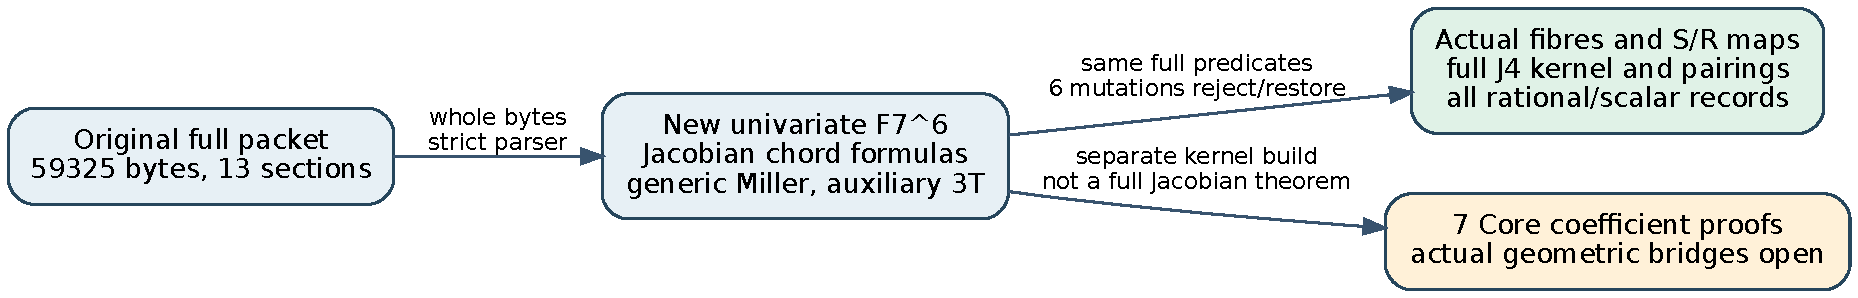
\includegraphics[width=\linewidth,height=48mm,keepaspectratio]{audit.pdf}
\end{center}

\textbf{Different arithmetic.} Work in
$R=\mathbb F_7[z]/(z^6+2z^4+5z^3+3z^2+6z+3)$ using coefficient
convolution and long reduction. With $A=z^3+4z+6$, $D=3z^2+5$,
$V=2z^4+3z^2+3z+1$, the identities $A^2-3D^2=m$ and $DV=1+6m$
give $b=AV$, $a=z-b$, $b^2=3$, $a^3+2a+6=0$. The known cubic
tower is a field and maps unitally into the six-dimensional quotient;
equal dimensions give the field isomorphism. A full-rank basis check
precedes Fermat inversion. The verifier uses Jacobian-coordinate chord
formulas and a generic two-doubling Miller loop with $3T=(5,1)$,
distinct from the producer's affine/closed-form evaluation at $T,2T$.

\textbf{Whole decisions without search replay.} The six marked division
roots are distinct and satisfy the monic degree-six polynomial. Its
degree bound exhausts the roots, certifying every unmarked bit while
evaluating only those six field elements. Every header, section,
coefficient, point, padding and completion byte is consumed.

\begin{center}
\begin{tabular}{lr>{\raggedright\arraybackslash}p{81mm}}
\toprule
Fixed original cohort & Count & Independent qualification\\
\midrule
Division-factor decisions &117649& Whole bitset; six-root degree bound\\
Actual $E_7[4]$ &16& Curve, full group, Frobenius and fixed basis\\
Actual Weil4 pairings &256& Generic Miller/third auxiliary; all stored values\\
Fibre/jet schemes &15& Complete degree2/3 quotient algebras, curve/forward/$R$\\
Actual $J[4]$ maps &4096& Every $S/R$/Frobenius/kernel record\\
Mixed kernel / pairings &64 /4096& Type$(4,4,2,2)$; Frobenius stable/isotropic\\
Rational Jacobian maps &1331& Bijections and both composites$[4]$\\
Original elliptic scalars &11& Full inclusion, transfer and recovery records\\
\bottomrule
\end{tabular}
\end{center}

The actual geometric $\beta:E_7^3\to\operatorname{Jac}(C_7)$ remains
the cited upstream bridge. The new fixed integer computations check
$S^*HS=R^*HR=4H$, $RS=SR=4I$, $Sv=u$, $\ell u=1$,
$\ell H^{-1}\ell^*=4$ and the actual pushforward row. The finite
coordinate tables are actual Jacobian tables through $\beta$; they do
not supply an arbitrary genus-three divisor reduction engine.
\newpage
{\Large\bfseries Partial proofs, negatives and exact next work}\par
\textbf{Seven checked coefficient leaves.} Lean4.35.0 builds the exact
Init-only source under120seconds/2GiB with the previously successful
InitG startup profile and explicit one-worker CLI setting. Both version
and proof phases exit zero, guards unchanged. Data3d0b82.

\begin{center}
\begin{tabular}{>{\raggedright\arraybackslash}p{76mm}>{\raggedright\arraybackslash}p{83mm}}
\toprule
Closed coefficient statement & Actual printed foundations\\
\midrule
$Sv=u$, $\ell u=1$, inverse Gram row & No axioms (three declarations)\\
Norm4 and numerator of $3L$ & No axioms (two declarations)\\
$A^2-3D^2=m$ and $DV=1+6m$ & Standard \texttt{propext} (two declarations)\\
\bottomrule
\end{tabular}
\end{center}

The field-quotient instance/evaluation, actual CM Hom action,
$\beta/\alpha$ inverse, Rosati transport and Jacobian/curve push-pull
remain unformalized. These closed arithmetic leaves do not replace that
full theorem. There is no \texttt{sorry}, custom research axiom or
\texttt{native\_decide} in the source. \texttt{lean4checker} is unavailable.
No unchanged failed Mathlib import was retried.

\textbf{Actual negative controls.} A scan bit, Weil$(4,6)$ value,
$J[4]$ $S$ target and $f_0$ fibre coefficient each fail their actual
predicate. A section-count and footer mutation fail the strict parser.
Each original whole packet is accepted again. The integer CM controls
also alter real $S/H$ coefficients and restore the original identities.

\textbf{First failures preserved.} SourceA\texttt{8278b6d} passed
versions/format but the compiler rejected an unused CM helper with
warnings denied;27 complete original files/448-byte diagnostic remain.
SourceB removes only that unused method and changes the CM module path.
FormalA aborted at \texttt{--version} before any proof build, with14
original files/132-byte thread diagnostic. A first claim's15-file
overcount is explicitly corrected by ac68db. FormalB corrects the caller
under the same toolchain/logical/resource bounds. No frozen A evidence
or predicate was rewritten.

\textbf{Source, raw and custody.} Frozen B \texttt{54f7e789} had all 59
input/lock files and every changed source, negative and metadata file read
back before calls: 103 complete files. Result \texttt{f66fea69} publishes
all 68 result files with full byte readback. Native stdout is 7867 bytes,
SHA256\texttt{4521481e\ldots{}b8810b}; 39 native and 18 formal small
originals remain complete. Original whole 4705736-byte executed ELF
\texttt{a9be75bc\ldots{}cf15b0} and 331888-byte olean
\texttt{c9c98bf4\ldots{}bfbba6} remain in RAM pending approved custody.

\textbf{Prime-field and algorithmic scope.} The degree-six field computes
geometric torsion; the maps are defined over$\mathbb F_7$. This is no
proper-subfield DLP descent or measured computational advantage. The
earlier written Hom gives a degree4 cover primitive over$\mathbb F_7$;
its rational functions remain unknown. Inverse3mod11 instead gives
global$[12]L$, a degree576 curve map agreeing on rational points.
Next compute exact pole/fibre divisor classes, then genuine function-field
functions, arbitrary target evaluation and fully charged algorithm costs.

\textbf{CI and continuation.} Focused ready-PR native/Core regression is
prepared separately and has not run. Crypto PR5080 first current-head CI
has 24 all-attempt checks/22 runs/four failures, with full diagnostics
recorded 76a6c6. No rerun/waiver or all-CI-green claim. Main-base required
gates, parent ledger fork and signed review stay separate.

\href{https://github.com/isogeny-labs/cryptanalysis/tree/54f7e78915475c6a989dd486c1dc0f3e3f0a6ea7/research/chained_cm19_univariate_audit_20261123}{Frozen source, protocol and first negatives}.\par
\href{https://github.com/isogeny-labs/cryptanalysis/tree/f66fea690e4be44306786e66516b59a1a1b5d078/research/chained_cm19_univariate_audit_20261123}{Complete result, native records and partial proofs}.\par
KB/Conductor unavailable; no novelty clearance. Vault/STOP/EKS ownership
unchanged. [pcc:unverified]
\end{document}
